\section{Finding the Optimal Classifiers}
\label{sec:algo}

\subsection{An Entropic Regularization}
\label{sec:entropic-reg}


% From now on, we focus on finite class of classifiers. Let $\Theta = \{\theta_1,\dots,\theta_K\}$, we aim to learn the optimal mixture of classifiers in this case. The adversarial risk  is defined as:
% \begin{align*}
%     \risk^\varepsilon(\lambda)=\mathbb{E}_{(x,y)\sim \PP}\left[\sup_{x'\in\mathcal{X},~d(x,x')\leq\varepsilon}\sum_{k=1}^K\lambda_kl(\theta_k,(x',y))\right]
% \end{align*}
% for $\lambda\in\Delta_K: = \{\lambda\in\mathbb{R}_+^K~\mathrm{s.t.}~\sum_{i=1}^K\lambda_i=1\}$, the probability simplex of $\mathbb{R}^K$. One can notice $\risk^\varepsilon(\cdot)$ is a continuous convex function, hence $\min_{\lambda\in\Delta_K}\risk^\varepsilon(\lambda)$ is attained for a certain $\lambda^*$. Then, thanks to Corollary XXX, there always exists a Nash equilbrium to the advarsarial game when $\Theta$ is finite. In this section, we present two algorithms to learn the find the optimum of the adversarial risk minimization problem.
% \subsection{Algorithm}
% The first algorithm we present is inspired from~\citep{sinha2017certifying} and the convergence of projected sub-gradient methods CITE. The computation of the inner supremum problem is usually NP-hard~\footnote{See App XXX for details.}, but one may assume the existence of an approximate oracle to this supremum. The algorithm is presented in Algorithm~\ref{algo:duchi}. We get the following guarantees on this algorithm. See proof in Appendix XXX.
% \begin{prop}
% Let $\PP\in\mathcal{M}^1_+(\mathcal{X}\times\mathcal{Y})$. Let $l:\Theta\times(\mathcal{X}\times\mathcal{Y})\to [0,\infty)$ satisfying Assumption~\ref{ass:loss}. Then, Algorithm~\ref{algo:duchi} satisfies:  
% \begin{align*}
%     \min_{t\in[T]}\risk^\varepsilon(\lambda_t)-\risk^\varepsilon(\lambda^*)\leq2\delta+ 2\sqrt{\frac{M}{T}}
%     % \delta\sqrt{K}+ \frac{M\sum_{t=1}^T \eta_t^2+\rVert\lambda_0-\lambda^*\lVert^2}{\sum_{t=1}^T\eta_t}
% \end{align*}
% % In particular for $\eta_t =\frac{\eta}{t^{1/2}}$, we get: $\min_{t\in[T]}\risk^\varepsilon(\lambda_t)-\risk^\varepsilon(\lambda^*)\in O\left(\delta+\frac{\log T}{\sqrt{T}}\right)$
% \end{prop}
% \begin{algorithm}[H]
% \SetAlgoLined
%  $\lambda_0 = \frac{\mathbf{1}_K}{K}; T;~\eta = \sqrt{\frac{4}{MT}}$\\
%  \For{$t=1,\dots,T$}{

%   $\Tilde{\QQ}$ s.t. $\exists\QQ^*\in\mathcal{A}_\varepsilon(\PP)$,  $\mathbb{E}_{\QQ^*,\lambda}(l(\theta_k,(x,y)))= \max_{\QQ\in \mathcal{A}_\varepsilon(\PP)}\mathbb{E}_{\QQ,\lambda}(l(\theta_k,(x,y)))$ and for all $k\in[K]$, $\lvert\mathbb{E}_{\Tilde{\QQ}}(l(\theta_k,(x,y)))-\mathbb{E}_{\QQ^*}(l(\theta_k,(x,y))) \rvert\leq\delta$\\
  
%   $g_t=\left(\mathbb{E}_{\Tilde{\QQ}}(l(\theta_1,(x,y)),\dots,\mathbb{E}_{\Tilde{\QQ}}(l(\theta_K,(x,y))\right)^T$\\
%   $\lambda_t = \Pi_{\Delta_K}\left(\lambda_{t-1}-\eta g_t\right)$
%   }
%  \caption{Mixture optimization by PGD}
 
%  \label{algo:duchi}

% \end{algorithm}
% \subsection{Entropic regularization}
Let $\{(x_i,y_i)\}_{i=1}^\numsamples$ samples independently drawn from $\PP$ and denote  $\widehat{\mathbb
{P}}:=\frac{1}{\numsamples}\sum_{i=1}^\numsamples \delta_{(x_i,y_i)}$ the associated empirical distribution. %In fact for such distribution we have a simple characterization of the set  of adversarial distributions which is:
% \begin{align*}
%     \mathcal{A}_{\varepsilon}&(\widehat{\mathbb
% {P}})=\Big\{\QQ~|\exists \QQ_1,\dots,\QQ_N\in\mathcal{M}_{+}(\mathcal{X}\times\mathcal{Y}),\QQ=\sum_{i=1}^N \QQ_i,\\
% & \int_{\mathcal{X}\times\mathcal{Y}}d\QQ_i=\frac{1}{N},~\int c_{\varepsilon}((x_i,y_i),\cdot)d\QQ_i=0\Big\}.
% \end{align*}
% where 
% \begin{align*}
% \delta_{B((x_i,y_i),\varepsilon)}(x,y) = \left\{
%     \begin{array}{ll}
%         0 & \mbox{if } d(x_i,x)\leq\varepsilon\mbox{ and }y_i = y\\
%         +\infty & \mbox{otherwise.}
% %     \end{array}
% % \right.
% % \end{align*}
% Therefore by denoting
% \begin{align*}
%     \Gamma_{\varepsilon}&(\widehat{\mathbb
%  {P}})=\Big\{(\QQ_1,\dots,\QQ_N)\mid\lvert \QQ_i\rvert =\frac{1}{N},~\int c_{\varepsilon}((x_i,y_i),\cdot)d\QQ_i=0\Big\}
% \end{align*}
% the problem of interest can be written as
% \begin{align*}
% \inf_{\mu\in \mathcal{M}^+_1(\Theta)}\sup_{(Q_1,\dots,Q_N)\in\Gamma_{\varepsilon}(\widehat{\mathbb
% {P}})}\sum_{i=1}^N\mathbb{E}_{(x,y)\sim Q_i,\theta \sim \mu}\left[\loss(\theta,(x,y))\right]
% \end{align*}
One can show the adversarial empirical risk minimization can be casted as:
\begin{align*}
\widehat{\mathcal{R}}_{adv}^{\varepsilon,*}:=\inf_{\mu\in \mathcal{M}^+_1(\Theta)}\sum_{i=1}^\numsamples\sup_{\QQ_i\in\Gamma_{i,\varepsilon}}\mathbb{E}_{(x,y)\sim \QQ_i,\theta \sim \mu}\left[\loss(\theta,(x,y))\right]
\end{align*}
where $\Gamma_{i,\varepsilon}$ is defined as : 
\begin{align*}
    \Gamma_{i,\varepsilon}:=\Big\{\QQ_i\mid~\int d\QQ_i=\frac{1}{\numsamples},~\int c_{\varepsilon}((x_i,y_i),\cdot) d\QQ_i=0\Big\}.
\end{align*}
\begin{prop}
    Let $\hat{\PP}:=\frac1N\sum_{i=1}^N \delta_{(x_i,y_i)}$. Let $l$ be a loss satisfying Assumption~\ref{ass:loss}. Then we have:
    \begin{align*}
    \frac{1}{N}\sum_{i=1}^N\sup_{x,~d(x,x_i)\leq\varepsilon}\mathbb{E}_{\theta \sim \mu}\left[l(\theta,(x,y))\right]=\sum_{i=1}^N\sup_{\QQ_i\in\Gamma_{i,\varepsilon}}\mathbb{E}_{(x,y)\sim \QQ_i,\theta \sim \mu}\left[l(\theta,(x,y))\right]
    \end{align*}
    where $\Gamma_{i,\varepsilon}$ is defined as : 
    \begin{align*}
        \Gamma_{i,\varepsilon}:=\Big\{\QQ_i\mid~\int d\QQ_i=\frac{1}{N},~\int c_{\varepsilon}((x_i,y_i),\cdot) d\QQ_i=0\Big\}.
    \end{align*}\end{prop}
    
    \begin{proof}
    This proposition is a direct application of Proposition~\ref{prop:dro_adv} for diracs $\delta_{(x_i,y_i)}$.
    \end{proof}
    
In the following, we regularize the above objective by adding an entropic term to each inner supremum problem. Let $\bm{\alpha}:=(\alpha_i)_{i=1}^\numsamples\in\mathbb{R}_+^\numsamples$ such that for all $i\in\{1,\dots,\numsamples\}$, and let us consider the following optimization problem:
\begin{equation*}
\begin{aligned}
\label{eq-legendre-KL}
\widehat{\mathcal{R}}_{adv,\bm{\alpha}}^{\varepsilon,*}:=\inf_{\mu\in \mathcal{M}^+_1(\Theta)}\sum_{i=1}^\numsamples&\sup_{\QQ_i\in\Gamma_{i,\varepsilon}}\mathbb{E}_{ \QQ_i, \mu}\left[\loss(\theta,(x,y))\right]\\
&-\alpha_i\text{KL}\left(\QQ_i\Big|\Big|\frac{1}{\numsamples}\mathbb{U}_{(x_i,y_i)}\right)
\end{aligned}
\end{equation*}
where $\mathbb{U}_{(x,y)}$ is an arbitrary distribution of support equal to:
\begin{align*}
    S_{(x,y)}^{(\varepsilon)}:=\Big\{(x',y'):~\text{s.t.}~c_{\varepsilon}((x,y),(x',y'))=0\Big\},
\end{align*}
and for all $\QQ,\mathbb{U}\in\mathcal{M}_{+}(\mathcal{X}\times\mathcal{Y})$,
\begin{align*}
\text{KL}(\QQ||\mathbb{U}):=  \left\{
    \begin{array}{lll}
        \int\log(\frac{d\QQ}{d\mathbb{U}})d\QQ+|\mathbb{U}| - |\QQ| &  \mbox{if } \QQ\ll \mathbb{U}\\
        +\infty & \mbox{otherwise.}
    \end{array}
\right.
\end{align*}
Note that when $\bm{\alpha}=0$, we recover the problem of interest $\widehat{\mathcal{R}}_{adv,\bm{\alpha}}^{\varepsilon,*}=\widehat{\mathcal{R}}_{adv}^{\varepsilon,*}$. Moreover, we show the regularized supremum tends to the standard supremum when $\bm{\alpha}\to 0$.
\begin{prop}
\label{prop:limit-eps}
For $\mu\in\mathcal{M}_{1}^{+}(\Theta)$, one has
\begin{align*}
    &\lim_{\alpha_i\rightarrow 0}\sup_{\QQ_i\in\Gamma_{i,\varepsilon}}\mathbb{E}_{\QQ_i,\mu}\left[\loss(\theta,(x,y))\right]-\alpha_i\text{KL}\left(\QQ\Big|\Big|\frac{1}{\numsamples}\mathbb{U}_{(x_i,y_i)}\right)\\
    &=\sup_{\QQ_i\in\Gamma_{i,\varepsilon}}\mathbb{E}_{(x,y)\sim \QQ_i,\theta \sim \mu}\left[\loss(\theta,(x,y))\right].
\end{align*}
\end{prop}
\begin{proof}
Let us first show that for $\alpha\geq 0$, $\sup_{\QQ_i\in\Gamma_{i,\varepsilon}}\mathbb{E}_{\QQ_i,\mu}\left[\loss(\theta,(x,y))\right]-\alpha\text{KL}\left(\QQ_i\Big|\Big|\frac{1}{\numsamples}\mathbb{U}_{(x_i,y_i)}\right)$ admits a solution. Let $\alpha\geq 0$,
$(\QQ_{\alpha,i}^{n})_{n\geq 0}$ a sequence such that
\begin{align*}
  \mathbb{E}_{\QQ_{\alpha,i}^{n},\mu}\left[\loss(\theta,(x,y))\right]&-\alpha\text{KL}\left(\QQ_{\alpha,i}^{n}\Big|\Big|\frac{1}{\numsamples}\mathbb{U}_{(x_i,y_i)}\right)\\
  &\xrightarrow[n]{} \sup_{\QQ_i\in\Gamma_{i,\varepsilon}}\mathbb{E}_{\QQ_i,\mu}\left[\loss(\theta,(x,y))\right]-\alpha\text{KL}\left(\QQ_i\Big|\Big|\frac{1}{\numsamples}\mathbb{U}_{(x_i,y_i)}\right).
\end{align*}
As $\Gamma_{i,\varepsilon}$ is tight ($(\mathcal{X},d)$ is a proper metric space therefore all the closed ball are compact) and by Prokhorov's theorem, we can extract a subsequence which converges  toward  $\QQ^{*}_{\alpha,i}$. Moreover, $\loss$ is upper semi-continuous (u.s.c), thus $\QQ\rightarrow \mathbb{E}_{\QQ,\mu}\left[\loss(\theta,(x,y))\right]$ is also u.s.c.\footnote{Indeed by considering a decreasing sequence of continuous and bounded functions which converge towards $\mathbb{E}_{\mu}\left[\loss(\theta,(x,y))\right]$ and by definition of the weak convergence the result follows.} Moreover 
$\QQ\rightarrow - \alpha \text{KL}\left(\QQ\Big|\Big|\frac{1}{\numsamples}\mathbb{U}_{(x_i,y_i)}\right)$ is also u.s.c. \footnote{for $\alpha=0$ the result is clear, and if $\alpha>0$, note that $\text{KL}\left(\cdot\Big|\Big|\frac{1}{\numsamples}\mathbb{U}_{(x_i,y_i)}\right)$ is lower semi-continuous}, therefore, by considering the limit superior as $n$ goes to infinity we obtain that
\begin{align*}
    &\limsup_{n\to+\infty}\mathbb{E}_{\QQ_{\alpha,i}^{n},\mu}\left[\loss(\theta,(x,y))\right]-\alpha\text{KL}\left(\QQ_{\alpha,i}^{n}\Big|\Big|\frac{1}{\numsamples}\mathbb{U}_{(x_i,y_i)}\right)\\
    &=\sup_{\QQ_i\in\Gamma_{i,\varepsilon}}\mathbb{E}_{\QQ_i,\mu}\left[\loss(\theta,(x,y))\right]-\alpha\text{KL}\left(\QQ_i\Big|\Big|\frac{1}{\numsamples}\mathbb{U}_{(x_i,y_i)}\right)\\
    &\leq \mathbb{E}_{\QQ_{\alpha,i}^{*},\mu}\left[\loss(\theta,(x,y))\right]-\alpha\text{KL}\left(\QQ_{\alpha,i}^{*}\Big|\Big|\frac{1}{\numsamples}\mathbb{U}_{(x_i,y_i)}\right)
\end{align*}
from which we deduce that $\QQ_{\alpha,i}^{*}$ is optimal.

Let us now show the result. We consider a positive sequence of $(\alpha_i^{(\ell)})_{\ell\geq0}$ such that $\alpha_i^{(\ell)}\to 0$.
Let us denote $\QQ^{*}_{\alpha_i^{(\ell)},i}$ and $\QQ^{*}_i$ the solutions of  $\max_{\QQ_i\in\Gamma_{i,\varepsilon}}\mathbb{E}_{\QQ_i,\mu}\left[\loss(\theta,(x,y))\right]-\alpha_i^{(\ell)}\text{KL}\left(\QQ_i\Big|\Big|\frac{1}{\numsamples}\mathbb{U}_{(x_i,y_i)}\right)$
and 
$\max_{\QQ_i\in\Gamma_{i,\varepsilon}}\mathbb{E}_{\QQ_i,\mu}\left[\loss(\theta,(x,y))\right]$ respectively.  Since $\Gamma_{i,\varepsilon}$ is tight, $(\QQ^{*}_{\alpha_i^{(\ell)},i})_{\ell\geq 0}$ is also tight and we can extract by Prokhorov's theorem a subsequence which converges towards $\QQ^{*}$. Moreover we have
\begin{align*}
 \mathbb{E}_{\QQ^{*}_i,\mu}\left[\loss(\theta,(x,y))\right] &-\alpha_i^{(\ell)}\text{KL}\left(\QQ^{*}_i\Big|\Big|\frac{1}{\numsamples}\mathbb{U}_{(x_i,y_i)}\right)\\
 &\leq \mathbb{E}_{\QQ^{*}_{\alpha_i^{(\ell)},i},\mu}\left[\loss(\theta,(x,y))\right] -\alpha_i^{(\ell)}\text{KL}\left(\QQ^{*}_{\alpha_i^{(\ell)},i}\Big|\Big|\frac{1}{\numsamples}\mathbb{U}_{(x_i,y_i)}\right)
\end{align*}
from which follows that
\begin{align*}
0\leq \mathbb{E}_{\QQ^{*}_i,\mu}\left[\loss(\theta,(x,y))\right] &-  \mathbb{E}_{\QQ^{*}_{\alpha_i^{(\ell)},i},\mu}\left[\loss(\theta,(x,y))\right]\\
&\leq \alpha_i^{(\ell)}\left(\text{KL}\left(\QQ^{*}_i\Big|\Big|\frac{1}{\numsamples}\mathbb{U}_{(x_i,y_i)}\right)- \text{KL}\left(\QQ^{*}_{\alpha_i^{(\ell)},i}\Big|\Big|\frac{1}{\numsamples}\mathbb{U}_{(x_i,y_i)}\right)\right)
\end{align*}
Then by considering the limit superior we obtain that
\begin{align*}
    \limsup_{\ell\to+\infty}\mathbb{E}_{\QQ^{*}_{\alpha_i^{(\ell)},i},\mu}\left[\loss(\theta,(x,y))\right] = \mathbb{E}_{\QQ^{*}_i,\mu}\left[\loss(\theta,(x,y))\right].
\end{align*}
from which follows that 
\begin{align*}
 \mathbb{E}_{\QQ^{*}_i,\mu}\left[\loss(\theta,(x,y))\right]\leq \mathbb{E}_{\QQ^{*},\mu}\left[\loss(\theta,(x,y))\right]
\end{align*}
and by optimality of $\QQ^{*}_i$ we obtain the desired result. 
\end{proof}



By adding an entropic term to the objective, we obtain an explicit formulation of the supremum involved in the sum: as soon as $\bm{\alpha}>0$ (which means that each $\alpha_i>0$), each sub-problem becomes just the Fenchel-Legendre transform of $\text{KL}(\cdot|\mathbb{U}_{(x_i,y_i)}/\numsamples)$ which has the following closed form:
\begin{align*}
 &\sup_{\QQ_i\in\Gamma_{i,\varepsilon}}\mathbb{E}_{\QQ_i, \mu}\left[\loss(\theta,(x,y))\right]-\alpha_i\text{KL}\left(\QQ_i||\frac{1}{\numsamples}\mathbb{U}_{(x_i,y_i)}\right)\\
 &=\frac{\alpha_i}{\numsamples}\log\left( \int_{\mathcal{X}\times\mathcal{Y}}\exp\left(\frac{\mathbb{E}_{\theta \sim \mu}\left[\loss(\theta,(x,y))\right]}{\alpha_i}\right)d\mathbb{U}_{(x_i,y_i)}\right).
\end{align*}
Finally, we end up with the following problem: 
\begin{align*}
  \inf_{\mu\in \mathcal{M}^+_1(\Theta)}\sum_{i=1}^\numsamples  \frac{\alpha_i}{\numsamples}\log\left( \int\exp\frac{\mathbb{E}_{ \mu}\left[\loss(\theta,(x,y))\right]}{\alpha_i}d\mathbb{U}_{(x_i,y_i)}\right).
\end{align*}
In order to solve the above problem, one needs to compute the integral involved in the objective. To do so, we estimate it by randomly sampling $m_i\geq 1$ samples $(u_1^{(i)},\dots,u_{m_i}^{(i)})\in(\mathcal{X}\times\mathcal{Y})^{m_i}$ from $\mathbb{U}_{(x_i,y_i)}$ for all $i\in\{1,\dots,\numsamples\}$ which leads to the following optimization problem
\begin{align}
\label{eq-obj-sample}
  \inf_{\mu\in \mathcal{M}^+_1(\Theta)}\sum_{i=1}^\numsamples  \frac{\alpha_i}{\numsamples}\log\left( \frac{1}{m_i}\sum_{j=1}^{m_i}\exp\frac{\mathbb{E}_{ \mu}\left[\loss(\theta,u_j^{(i)})\right]}{\alpha_i}\right)
\end{align}
denoted $\widehat{\mathcal{R}}_{adv,\bm{\alpha}}^{\varepsilon,\bm{m}}$ where $\bm{m}:=(m_i)_{i=1}^\numsamples$ in the following. Now we aim at controlling the error made with our approximations. We decompose the error into two terms
\begin{align*}
  |\widehat{\mathcal{R}}_{adv,\bm{\alpha}}^{\varepsilon,\bm{m}} - \widehat{\mathcal{R}}_{adv}^{\varepsilon,*}|
   \leq |\widehat{\mathcal{R}}_{adv,\bm{\alpha}}^{\varepsilon,*} - \widehat{\mathcal{R}}_{adv,\bm{\alpha}}^{\varepsilon,\bm{m}}| +|\widehat{\mathcal{R}}_{adv,\bm{\alpha}}^{\varepsilon,*} - \widehat{\mathcal{R}}_{adv}^{\varepsilon,*}|
\end{align*}
where the first one corresponds to the statistical error made by our estimation of the integral, and the second to the approximation error made by the entropic regularization of the objective. First, we show a control of the statistical error using Rademacher complexities~\citep{bartlett2002rademacher}. %See proof in Appendix~\ref{prv:control-error-stat}.
\begin{prop}
\label{prop:control-error-stat}
Let $m\geq 1$ and $\alpha>0$ and denote $\bm{\alpha}:=(\alpha,\dots,\alpha)\in\mathbb{R}^\numsamples$ and $\bm{m}:=(m,\dots,m)\in\mathbb{R}^\numsamples$.  \textcolor{black}{Then by denoting $\tilde{M}=\max(M,1)$}, we have with a probability of at least $1-\delta$
\begin{align*}
|\widehat{\mathcal{R}}_{adv,\bm{\alpha}}^{\varepsilon,*} - \widehat{\mathcal{R}}_{adv,\bm{\alpha}}^{\varepsilon,\bm{m}}|\leq& \frac{2e^{M/\alpha}}{\numsamples}\sum_{i=1}^\numsamples R_i + \color{black}{6\tilde{M}}\color{black}e^{M/\alpha}\sqrt{\frac{\log(\frac4\delta)}{2m\numsamples}}
\end{align*}
where $R_i:=\frac{1}{m}\mathbb{E}_{\bm{\sigma}}\left[\sup_{\theta\in\Theta}\sum_{j=1}^m \sigma_j l(\theta,u_j^{(i)})\right]$ and $\bm{\sigma}:=(\sigma_1,\dots,\sigma_m)$ with $\sigma_i$ i.i.d. sampled as $\mathbb{P}[\sigma_i=\pm1]=1/2$.
\end{prop}

\begin{proof}
Let us denote for all $\mu\in\mathcal{M}_1^{+}(\Theta)$,
\begin{align*}
  \widehat{\mathcal{R}}^{\bm{\varepsilon},\textbf{m}}_{adv,\bm{\alpha}}(\mu):=  \sum_{i=1}^\numsamples  \frac{\alpha_i}{\numsamples}\log\left( \frac{1}{m_i}\sum_{j=1}^{m_i}\exp\frac{\mathbb{E}_{ \mu}\left[\loss(\theta,u_j^{(i)})\right]}{\alpha_i}\right).
\end{align*}
Let also consider $(\mu^{(\textbf{m})}_n)_{n\geq 0}$ and $(\mu_n)_{n\geq 0}$ two sequences such that
\begin{align*}
 \widehat{\mathcal{R}}^{\bm{\varepsilon},\textbf{m}}_{adv,\bm{\alpha}}(\mu^{(\textbf{m})}_n) \xrightarrow[n \to +\infty]{}\widehat{\mathcal{R}}^{\bm{\varepsilon},\textbf{m}}_{adv,\bm{\alpha}},~\quad
\widehat{\mathcal{R}}^{\bm{\varepsilon}}_{adv,\bm{\alpha}}(\mu_n)\xrightarrow[n \to +\infty]{}\widehat{\mathcal{R}}^{\bm{\varepsilon},*}_{adv,\bm{\alpha}}.
\end{align*}
We first remarks that
\begin{align*}
\widehat{\mathcal{R}}^{\bm{\varepsilon},\textbf{m}}_{adv,\bm{\alpha}}- \widehat{\mathcal{R}}^{\bm{\varepsilon},*}_{adv,\bm{\alpha}}&\leq \widehat{\mathcal{R}}^{\bm{\varepsilon},\textbf{m}}_{adv,\bm{\alpha}} - \widehat{\mathcal{R}}^{\bm{\varepsilon},\textbf{m}}_{adv,\bm{\alpha}}(\mu_n)\\
& + \widehat{\mathcal{R}}^{\bm{\varepsilon},\textbf{m}}_{adv,\bm{\alpha}}(\mu_n) - \widehat{\mathcal{R}}^{\bm{\varepsilon}}_{adv,\bm{\alpha}}(\mu_n)\\
&+ \widehat{\mathcal{R}}^{\bm{\varepsilon}}_{adv,\bm{\alpha}}(\mu_n)-
\widehat{\mathcal{R}}^{\bm{\varepsilon},*}_{adv,\bm{\alpha}} \\
&\leq \sup_{\mu\in \mathcal{M}^+_1(\Theta)}\Big|\widehat{\mathcal{R}}^{\bm{\varepsilon},\textbf{m}}_{adv,\bm{\alpha}}(\mu) - \widehat{\mathcal{R}}^{\bm{\varepsilon}}_{adv,\bm{\alpha}}(\mu) \Big|\\
& + \widehat{\mathcal{R}}^{\bm{\varepsilon}}_{adv,\bm{\alpha}}(\mu_n)-
\widehat{\mathcal{R}}^{\bm{\varepsilon},*}_{adv,\bm{\alpha}},
\end{align*}
and by considering the limit, we obtain that
\begin{align*}
  \widehat{\mathcal{R}}^{\bm{\varepsilon},\textbf{m}}_{adv,\bm{\alpha}}- \widehat{\mathcal{R}}^{\bm{\varepsilon},*}_{adv,\bm{\alpha}}&\leq  \sup_{\mu\in \mathcal{M}^+_1(\Theta)}\Big|\widehat{\mathcal{R}}^{\bm{\varepsilon},\textbf{m}}_{adv,\bm{\alpha}}(\mu) - \widehat{\mathcal{R}}^{\bm{\varepsilon}}_{adv,\bm{\alpha}}(\mu) \Big| 
\end{align*}
Simarly we have that
\begin{align*}
\widehat{\mathcal{R}}^{\bm{\varepsilon},*}_{adv,\bm{\alpha}} - \widehat{\mathcal{R}}^{\bm{\varepsilon},\textbf{m}}_{adv,\bm{\alpha}}&\leq \widehat{\mathcal{R}}^{\bm{\varepsilon},*}_{adv,\bm{\alpha}} -
\widehat{\mathcal{R}}^{\bm{\varepsilon}}_{adv,\bm{\alpha}}(\mu_n^{(\bm{m})})\\
&+\widehat{\mathcal{R}}^{\bm{\varepsilon}}_{adv,\bm{\alpha}}(\mu_n^{(\bm{m})}) - \widehat{\mathcal{R}}^{\bm{\varepsilon},\textbf{m}}_{adv,\bm{\alpha}}(\mu_n^{(\bm{m})}) \\
&+ \widehat{\mathcal{R}}^{\bm{\varepsilon},\textbf{m}}_{adv,\bm{\alpha}}(\mu_n^{(\bm{m})}) - \widehat{\mathcal{R}}^{\bm{\varepsilon},\textbf{m}}_{adv,\bm{\alpha}}
\end{align*}
from which follows that 
\begin{align*}
\widehat{\mathcal{R}}^{\bm{\varepsilon},*}_{adv,\bm{\alpha}} - \widehat{\mathcal{R}}^{\bm{\varepsilon},\textbf{m}}_{adv,\bm{\alpha}}&\leq  \sup_{\mu\in \mathcal{M}^+_1(\Theta)}\Big|\widehat{\mathcal{R}}^{\bm{\varepsilon},\textbf{m}}_{adv,\bm{\alpha}}(\mu) - \widehat{\mathcal{R}}^{\bm{\varepsilon}}_{adv,\bm{\alpha}}(\mu) \Big| 
\end{align*}
Therefore we obtain that 
\begin{align*}
\Big| \widehat{\mathcal{R}}^{\bm{\varepsilon},*}_{adv,\bm{\alpha}} - \widehat{\mathcal{R}}^{\bm{\varepsilon},\textbf{m}}_{adv,\bm{\alpha}}\Big |\leq 
\sum_{i=1}^\numsamples\frac{\alpha}{\numsamples}  &\sup_{\mu\in \mathcal{M}^+_1(\Theta)}\Big|\log\left(\frac{1}{m_i}\sum_{j=1}^{m_i}\exp\left(\frac{\mathbb{E}_{\theta \sim \mu}\left[\loss(\theta,u_j^{(i)}))\right]}{\alpha}\right)\right)\\
    &- \log\left(\int_{\mathcal{X}\times\mathcal{Y}}\exp\left(\frac{\mathbb{E}_{\theta \sim \mu}\left[\loss(\theta,(x,y))\right]}{\alpha}\right) d\mathbb{U}_{(x_i,y_i)} \right)\Big|.
\end{align*}
Observe that $\loss\geq 0$, therefore because the $\log$ function is 1-Lipschitz on $[1,+\infty)$, we obtain that 
\begin{align*}
\Big| \widehat{\mathcal{R}}^{\bm{\varepsilon},*}_{adv,\bm{\alpha}} - \widehat{\mathcal{R}}^{\bm{\varepsilon},\textbf{m}}_{adv,\bm{\alpha}}\Big |
\leq 
\sum_{i=1}^\numsamples\frac{\alpha}{\numsamples}  &\sup_{\mu\in \mathcal{M}^+_1(\Theta)}\Big |\frac{1}{m_i}\sum_{j=1}^{m_i}\exp\left(\frac{\mathbb{E}_{\theta \sim \mu}\left[\loss(\theta,u_j^{(i)}))\right]}{\alpha}\right)\\
    &- \int_{\mathcal{X}\times\mathcal{Y}}\exp\left(\frac{\mathbb{E}_{\theta \sim \mu}\left[\loss(\theta,(x,y))\right]}{\alpha}\right) d\mathbb{U}_{(x_i,y_i)} \Big|.
\end{align*}
Let us now denote for all $i=1,\dots,\numsamples$,
\begin{align*}
    \widehat{R}_i(\mu,\bm{u}^{(i)})&:=\sum_{j=1}^{m_i}\exp\left(\frac{\mathbb{E}_{\theta \sim \mu}\left[\loss(\theta,u_j^{(i)}))\right]}{\alpha}\right)\\
    R_i(\mu)&:= \int_{\mathcal{X}\times\mathcal{Y}}\exp\left(\frac{\mathbb{E}_{\theta \sim \mu}\left[\loss(\theta,(x,y))\right]}{\alpha}\right) d\mathbb{U}_{(x_i,y_i)}.
\end{align*}
and let us define 
\begin{align*}
    f(\bm{u}^{(1)},\dots,\bm{u}^{(\numsamples)}):=\sum_{i=1}^\numsamples\frac{\alpha}{\numsamples}\sup_{\mu\in \mathcal{M}^+_1(\Theta)}\Big |\widehat{R}_i(\mu) -R_i(\mu)\Big |
\end{align*}
where $\bm{u}^{(i)}:=(u_1^{(i)},\dots,u_1^{(m)})$. By denoting $z^{(i)}=(u_1^{(i)},\dots,u_{k-1}^{(i)},z,u_{k+1}^{(i)},\dots,u_m^{(i)})$, we have that
\begin{align*}
  |f(\bm{u}^{(1)},\dots,\bm{u}^{(\numsamples)})& - f(\bm{u}^{(1)},\dots,\bm{u}^{(i-1)},\bm{z}^{(i)},\bm{u}^{(i+1)},\dots,\bm{u}^{(\numsamples)})|\\
  &\leq \frac{\alpha}{\numsamples}\Big | \sup_{\mu\in \mathcal{M}^+_1(\Theta)}\Big |\widehat{R}_i(\mu,\bm{u}^{(i)}) -R_i(\mu)\Big |\\
 & - \sup_{\mu\in \mathcal{M}^+_1(\Theta)}\Big |\widehat{R}_i(\mu,\bm{z}^{(i)}) -R_i(\mu)\Big | \Big |\\
  &\leq \frac{\alpha}{\numsamples}\Big |\frac{1}{m}\left[\exp\left(\frac{\mathbb{E}_{\theta \sim \mu}\left[\loss(\theta,u_k^{(i)}))\right]}{\alpha}\right) - \exp\left(\frac{\mathbb{E}_{\theta \sim \mu}\left[\loss(\theta,z^{(i)}))\right]}{\alpha}\right) \right]\Big| \\
  &\leq \frac{2\exp(M/\alpha)}{\numsamples m}
\end{align*}
where the last inequality comes from the fact that the loss is upper bounded by $\loss\leq M$. Then by appling the McDiarmid’s Inequality, we obtain that with a probability of at least $1-\delta$,
\begin{align*}
 \Big| \widehat{\mathcal{R}}^{\bm{\varepsilon},*}_{adv,\bm{\alpha}} - \widehat{\mathcal{R}}^{\bm{\varepsilon},\textbf{m}}_{adv,\bm{\alpha}}\Big |\leq\mathbb{E}(f(\bm{u}^{(1)},\dots,\bm{u}^{(\numsamples)}))+\frac{2\exp(M/\alpha)}{\sqrt{m\numsamples}}\sqrt{\frac{\log(2/\delta)}{2}}.
\end{align*}
Thanks to~\citep[Lemma 26.2]{shalev2014understanding}, we have for all $i\in\{1,\dots,\numsamples\}$
\begin{align*}
\mathbb{E}(f(\bm{u}^{(1)},\dots,\bm{u}^{(\numsamples)}))\leq 2 \mathbb{E}(\text{Rad}(\mathcal{F}_i\circ \mathbf{u^{(i)}}))    
\end{align*}
where for any class of function $\mathcal{F}$ defined on $\mathcal{Z}$  and point $\bm{z}:(z_1,\dots,z_q)\in\mathcal{Z}^q$
\begin{align*}
    &\mathcal{F}\circ \bm{z}:=\Big\{(f(z_1),\dots,f(z_q)),f\in\mathcal{F}\Big\} \quad,\\\quad \text{Rad}(\mathcal{F}\circ \bm{z}):=\frac{1}{q}\mathbb{E}_{\bm{\sigma}\sim\{\pm 1\}}\left[\sup_{f\in\mathcal{F}}\sum_{i=1}^q\sigma_if(z_i)\right],\\
    &\mathcal{F}_i:=\Big\{u\rightarrow\exp\left(\frac{\mathbb{E}_{\theta \sim \mu}\left[\loss(\theta,u))\right]}{\alpha}\right),~\mu\in\mathcal{M}_{1}^{+}(\Theta) \Big\}.
      \end{align*}
Moreover as $x\rightarrow\exp(x/\alpha)$ is $\frac{\exp(M/\alpha)}{\alpha}$-Lipstchitz on $(-\infty,M]$, by~\citep[Lemma 26.9]{shalev2014understanding}, we have 
\begin{align*}
   \text{Rad}(\mathcal{F}_i\circ \mathbf{u^{(i)}})\leq \frac{\exp(M/\alpha)}{\alpha} \text{Rad}(\mathcal{H}_i\circ \mathbf{u^{(i)}}) 
\end{align*}
where 
\begin{align*}
    \mathcal{H}_i:=\Big\{u\rightarrow \mathbb{E}_{\theta \sim \mu}\left[\loss(\theta,u))\right],~\mu\in\mathcal{M}_{1}^{+}(\Theta) \Big\}.
\end{align*}
Let us now define
\begin{align*}
    g(\bm{u}^{(1)},\dots,\bm{u}^{(\numsamples)}):=\sum_{j=1}^\numsamples\frac{2\exp(M/\alpha)}{\numsamples}\text{Rad}(\mathcal{H}_j\circ \mathbf{u^{(j)}}).
\end{align*}
We observe that 
\begin{align*}
|g(\bm{u}^{(1)},\dots,\bm{u}^{(\numsamples)}) &- g(\bm{u}^{(1)},\dots,\bm{u}^{(i-1)},\bm{z}^{(i)},\bm{u}^{(i+1)},\dots,\bm{u}^{(\numsamples)})|\\
&\leq \frac{2\exp(M/\alpha)}{\numsamples}|\text{Rad}(\mathcal{H}_i\circ \mathbf{u^{(i)}}) - \text{Rad}(\mathcal{H}_i\circ \mathbf{z^{(i)}})|\\
&\leq \frac{2\exp(M/\alpha)}{\numsamples}\frac{2M}{m}.
\end{align*}
By Applying the McDiarmid’s Inequality, we have that with a probability of at least $1-\delta$
\begin{align*}
\mathbb{E}(g(\bm{u}^{(1)},\dots,\bm{u}^{(\numsamples)}))\leq g(\bm{u}^{(1)},\dots,\bm{u}^{(\numsamples)}) +\frac{4\exp(M/\alpha)M}{\sqrt{m\numsamples}}\sqrt{\frac{\log(2/\delta)}{2}}.
\end{align*}
Remarks also that 
\begin{align*}
    \text{Rad}(\mathcal{H}_i\circ \mathbf{u^{(i)}})&=\frac{1}{m}\mathbb{E}_{\bm{\sigma}\sim\{\pm 1\}}\left[\sup_{\mu\in\mathcal{M}_1^{+}(\Theta)}\sum_{j=1}^m\sigma_i\mathbb{E}_{\mu}(l(\theta,u^{(i)}_j))\right]\\
    &=\frac{1}{m}\mathbb{E}_{\bm{\sigma}\sim\{\pm 1\}}\left[\sup_{\theta\in\Theta}\sum_{j=1}^m\sigma_i l(\theta,u^{(i)}_j)\right]
\end{align*}
Finally, applying a union bound leads to the desired result.

\end{proof}




We deduce from the above Proposition that in the particular case where $\Theta$ is finite such that $|\Theta|= l$, with probability of at least $1-\delta$
\begin{align*}
   |\widehat{\mathcal{R}}_{adv,\bm{\alpha}}^{\varepsilon,*} - \widehat{\mathcal{R}}_{adv,\bm{\alpha}}^{\varepsilon,\bm{m}}| \in \mathcal{O}\left(Me^{M/\alpha}\sqrt{\frac{\log(l)}{m}} \right).
\end{align*}
This case is of particular interest when one wants to learn the optimal mixture of some given classifiers in order to minimize the adversarial risk. In the following proposition, we control the approximation error made by adding an entropic term to the objective. %See proof in Appendix~\ref{prv:control-error-approx}.
\begin{prop}
\label{prop:control-error-approx}
Denote for $\beta>0$, $(x,y)\in\mathcal{X}\times\mathcal{Y}$ and $\mu\in\mathcal{M}_{1}^{+}(\Theta)$,
    $$A_{\beta,\mu}^{\left(  x,y\right)}:=\{u|\sup_{v\in  S_{(x,y)}^{(\varepsilon)}}\mathbb{E}_{\mu}[\loss(\theta,v)]\leq \mathbb{E}_{\mu}[\loss(\theta,u)]+\beta\}$$. 
    If there exists $C_{\beta}$ such that for all $(x,y)\in\mathcal{X}\times\mathcal{Y}$ and $\mu\in\mathcal{M}_{1}^{+}(\Theta)$, $\mathbb{U}_{(x,y)}\left(A_{\beta,\mu}^{\left(  x,y\right)}\right)\geq C_\beta$ then we have
\begin{align*}
   |\widehat{\mathcal{R}}_{adv,\bm{\alpha}}^{\varepsilon,*} - \widehat{\mathcal{R}}_{adv}^{\varepsilon,*}|\leq 2\alpha |\log(C_\beta)| + \beta.
\end{align*}
\end{prop}




The assumption made in the above Proposition states that for any given random classifier $\mu$, and any given point $(x,y)$, the set of $\beta$-optimal attacks at this point has at least a certain amount of mass depending on the $\beta$ chosen. This assumption is always met when $\beta$ is sufficiently large. However in order to obtain a tight control of the error, a trade-off exists between $\beta$ and the smallest amount of mass $C_{\beta}$ of $\beta$-optimal attacks.

\begin{proof}
Following the same steps than the proof of Proposition~\ref{prop:control-error-stat}, let $(\mu_n^{\varepsilon})_{n\geq 0}$ and $(\mu_n)_{n\geq 0}$ two sequences such that
\begin{align*}
    \widehat{\mathcal{R}}_{adv,\bm{\alpha}}^{\varepsilon}(\mu_n^{\varepsilon})\xrightarrow[n \to +\infty]{}\widehat{\mathcal{R}}_{adv,\bm{\alpha}}^{\varepsilon,*},~\quad \widehat{\mathcal{R}}_{adv}^{\varepsilon}(\mu_n)\xrightarrow[n \to +\infty]{}\widehat{\mathcal{R}}_{adv}^{\varepsilon,*}.
\end{align*}
Remarks that 
\begin{align*}
  \widehat{\mathcal{R}}_{adv,\bm{\alpha}}^{\varepsilon,*} - \widehat{\mathcal{R}}_{adv}^{\varepsilon,*}&\leq \widehat{\mathcal{R}}_{adv,\bm{\alpha}}^{\varepsilon,*} - \widehat{\mathcal{R}}_{adv,\bm{\alpha}}^{\varepsilon}(\mu_n)\\
  & + \widehat{\mathcal{R}}_{adv,\bm{\alpha}}^{\varepsilon}(\mu_n) -   \widehat{\mathcal{R}}_{adv}^{\varepsilon}(\mu_n)\\
  &+ \widehat{\mathcal{R}}_{adv}^{\varepsilon}(\mu_n)-\widehat{\mathcal{R}}_{adv}^{\varepsilon,*}\\
  &\leq \sup_{\mu\in\mathcal{M}_1^{+}(\Theta)}\Big|\widehat{\mathcal{R}}_{adv,\bm{\alpha}}^{\varepsilon}(\mu) -   \widehat{\mathcal{R}}_{adv}^{\varepsilon}(\mu)  \Big|\\
  & + \widehat{\mathcal{R}}_{adv}^{\varepsilon}(\mu_n)-\widehat{\mathcal{R}}_{adv}^{\varepsilon,*}
\end{align*}
Then by considering the limit we obtain that 
\begin{align*}
    \widehat{\mathcal{R}}_{adv,\bm{\alpha}}^{\varepsilon,*} - \widehat{\mathcal{R}}_{adv}^{\varepsilon,*}&\leq \sup_{\mu\in\mathcal{M}_1^{+}(\Theta)}\Big|\widehat{\mathcal{R}}_{adv,\bm{\alpha}}^{\varepsilon}(\mu) -   \widehat{\mathcal{R}}_{adv}^{\varepsilon}(\mu)  \Big|.
\end{align*}
Similarly, we obtain that 
\begin{align*}
     \widehat{\mathcal{R}}_{adv}^{\varepsilon,*}-\widehat{\mathcal{R}}_{adv,\bm{\alpha}}^{\varepsilon,*}&\leq \sup_{\mu\in\mathcal{M}_1^{+}(\Theta)}\Big|\widehat{\mathcal{R}}_{adv,\bm{\alpha}}^{\varepsilon}(\mu) -   \widehat{\mathcal{R}}_{adv}^{\varepsilon}(\mu)  \Big|,
\end{align*}
from which follows that
\begin{align*}
 \Big| \widehat{\mathcal{R}}_{adv,\bm{\alpha}}^{\varepsilon,*} - \widehat{\mathcal{R}}_{adv}^{\varepsilon,*}\Big|\leq \frac{1}{\numsamples}\sum_{i=1}^\numsamples&\sup_{\mu\in\mathcal{M}_1^{+}(\Theta)}\Big|\alpha\log\left(\int_{\mathcal{X}\times\mathcal{Y}}\exp\left(\frac{\mathbb{E}_{\mu}[\loss(\theta,(x,y))]}{\alpha} \right) d\mathbb{U}_{(x_i,y_i)}\right)\\
 &-\sup_{u\in S^{\varepsilon}_{(x_i,y_i)}}\mathbb{E}_{\mu}[\loss(\theta,u)] \Big|.
\end{align*}
Let $\mu\in\mathcal{M}_1^{+}(\Theta)$ and $i\in\{1,\dots,\numsamples\}$, then we have
\begin{align*}
 \Big|\alpha&\log\left(\int_{\mathcal{X}\times\mathcal{Y}}\exp\left(\frac{\mathbb{E}_{\mu}[\loss(\theta,(x,y))]}{\alpha} \right) d\mathbb{U}_{(x_i,y_i)}\right)-\sup_{u\in S^{\varepsilon}_{(x_i,y_i)}}\mathbb{E}_{\mu}[\loss(\theta,u)] \Big|\\
 &=\Big|\alpha\log\left(\int_{\mathcal{X}\times\mathcal{Y}}\exp\left(\frac{\mathbb{E}_{\mu}[\loss(\theta,(x,y))]-\sup_{u\in S^{\varepsilon}_{(x_i,y_i)}}\mathbb{E}_{\mu}[\loss(\theta,u)]}{\alpha} \right) d\mathbb{U}_{(x_i,y_i)}\right) \Big|  \\
 &=\alpha  \Big| \log\left(\int_{A_{\beta,\mu}^{(x_i,y_i)}}\exp\left(\frac{\mathbb{E}_{\mu}[\loss(\theta,(x,y))]-\sup_{u\in S^{\varepsilon}_{(x_i,y_i)}}\mathbb{E}_{\mu}[\loss(\theta,u)]}{\alpha} \right) d\mathbb{U}_{(x_i,y_i)}\right. \\
 &+ \left.\int_{(A_{\beta,\mu}^{(x_i,y_i)})^{c}}\exp\left(\frac{\mathbb{E}_{\mu}[\loss(\theta,(x,y))]-\sup_{u\in S^{\varepsilon}_{(x_i,y_i)}}\mathbb{E}_{\mu}[\loss(\theta,u)]}{\alpha} \right) d\mathbb{U}_{(x_i,y_i)}\right)  \Big|\\
 &\leq \alpha \Big | \log\left(\exp(-\frac\beta\alpha)\mathbb{U}_{(x_i,y_i)}\left(A_{\beta,\mu}^{(x_i,y_i)}\right) \right)\Big | \\
 &+ \alpha  \Big|\log\left(1+\right.\\
 &\left.\frac{\exp(\beta/\alpha)}{\mathbb{U}_{(x_i,y_i)}\left(A_{\beta,\mu}^{(x_i,y_i)}\right)}\int_{(A_{\beta,\mu}^{(x_i,y_i)})^{c}}\exp\left(\frac{\mathbb{E}_{\mu}[\loss(\theta,(x,y))]-\sup_{u\in S^{\varepsilon}_{(x_i,y_i)}}\mathbb{E}_{\mu}[\loss(\theta,u)]}{\alpha} \right) d\mathbb{U}_{(x_i,y_i)}\right)  \Big|\\
 &\leq \alpha\log(1/C_\beta)+\beta +\frac{\alpha}{C_\beta}\\
 &\leq 2\alpha\log(1/C_\beta)+\beta
\end{align*}
\end{proof}



Now that we have shown that solving~\eqref{eq-obj-sample} allows to obtain an approximation of the true solution $\widehat{\mathcal{R}}_{adv}^{\varepsilon,*}$, we next aim at deriving an algorithm to compute it. 

\subsection{Proposed Algorithms}
\label{sec:proposed-algo}
From now on, we focus on finite class of classifiers. Let $\Theta = \{\theta_1,\dots,\theta_l\}$, we aim to learn the optimal mixture of classifiers in this case. The adversarial empirical risk  is therefore defined as:
\begin{align*}
    \widehat{\mathcal{R}}_{adv}^\varepsilon(\bm{\lambda})= \sum_{i=1}^\numsamples\sup_{\QQ_i\in\Gamma_{i,\varepsilon}}\mathbb{E}_{(x,y)\sim \QQ_i}\left[\sum_{k=1}^l \lambda_k \loss(\theta_k,(x,y))\right]
\end{align*}
for $\bm{\lambda}\in\Delta_l: = \{\bm{\lambda}\in\mathbb{R}_+^l~\mathrm{s.t.}~\sum_{i=1}^l\lambda_i=1\}$, the probability simplex of $\mathbb{R}^l$. One can notice that $ \widehat{\mathcal{R}}_{adv}^\varepsilon(\cdot)$ is a continuous convex function, hence $\min_{\bm{\lambda}\in\Delta_l}\risk^\varepsilon(\bm{\lambda})$ is attained for a certain $\bm{\lambda}^*$. Then there exists a non-approximate Nash equilibrium $(\bm{\lambda}^*,\QQ^*)$ in the adversarial game when $\Theta$ is finite. Here, we present two algorithms to learn the optimal mixture of the adversarial risk minimization problem.


\begin{algorithm}[ht]
\SetAlgoLined
 $\bm{\lambda}_0 = \frac{\mathbf{1}_L}{L}; T;~\textcolor{black}{\eta=\frac{2}{M\sqrt{LT}}}$\\
 \For{$t=1,\dots,T$}{

  $\Tilde{\QQ}$ s.t. $\exists\QQ^*\in\mathcal{A}_\varepsilon(\PP)$ best response to \textcolor{black}{$\bm{\lambda}_{t-1}$} and for all $k\in[L]$, $\lvert\mathbb{E}_{\Tilde{\QQ}}(l(\theta_k,(x,y)))-\mathbb{E}_{\QQ^*}(l(\theta_k,(x,y))) \rvert\leq\delta$\\
  $\bm{g}_t=\left(\mathbb{E}_{\Tilde{\QQ}}(l(\theta_1,(x,y)),\dots,\mathbb{E}_{\Tilde{\QQ}}(l(\theta_L,(x,y))\right)^T$\\
  $\bm{\lambda}_t = \Pi_{\Delta_L}\left(\bm{\lambda}_{t-1}-\eta \bm{g}_t\right)$
  }
 \caption{Oracle-based Algorithm}
 \label{algo:duchi}
\end{algorithm}
% To validate 
\begin{figure*}[!ht]
    \centering
    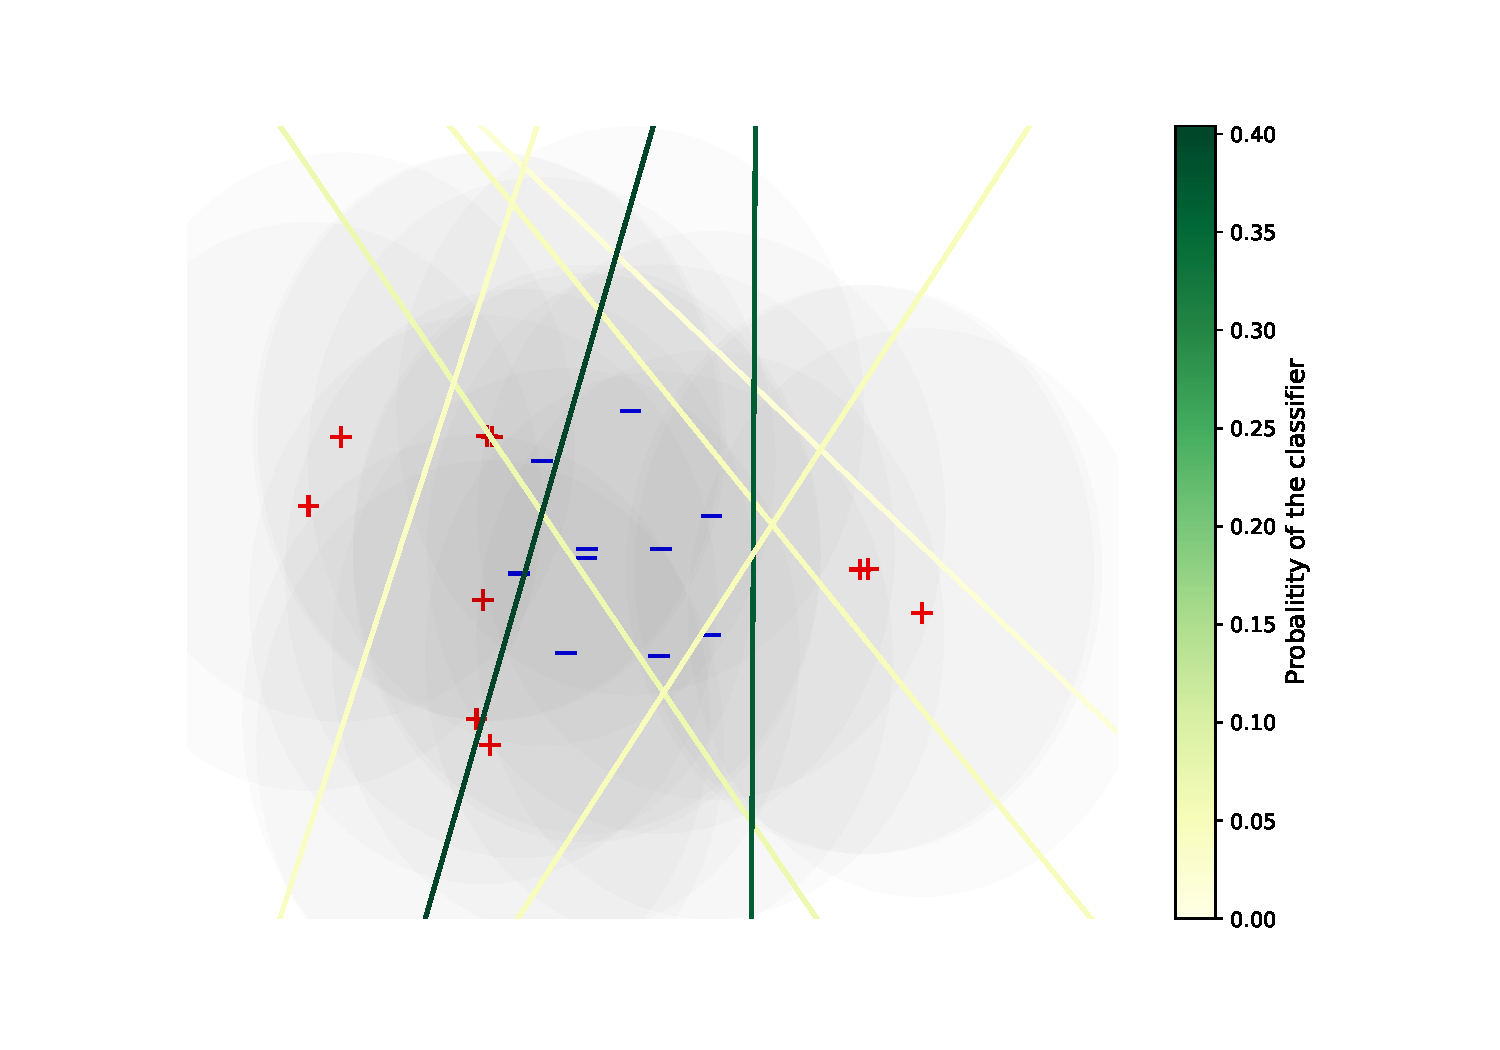
\includegraphics[width=0.32\textwidth]{Images/illustration.pdf}  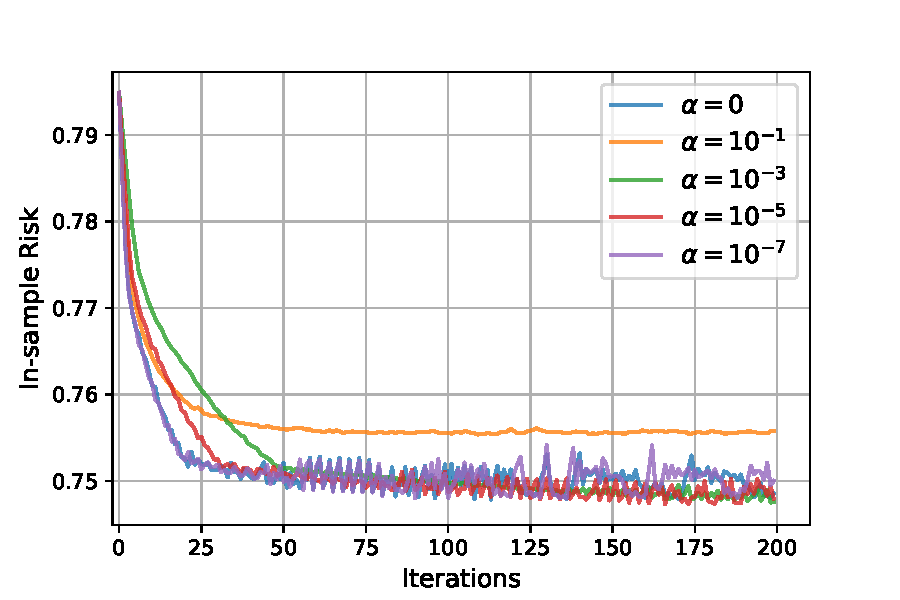
\includegraphics[width=0.32\textwidth]{Images/convergence_toy.pdf}     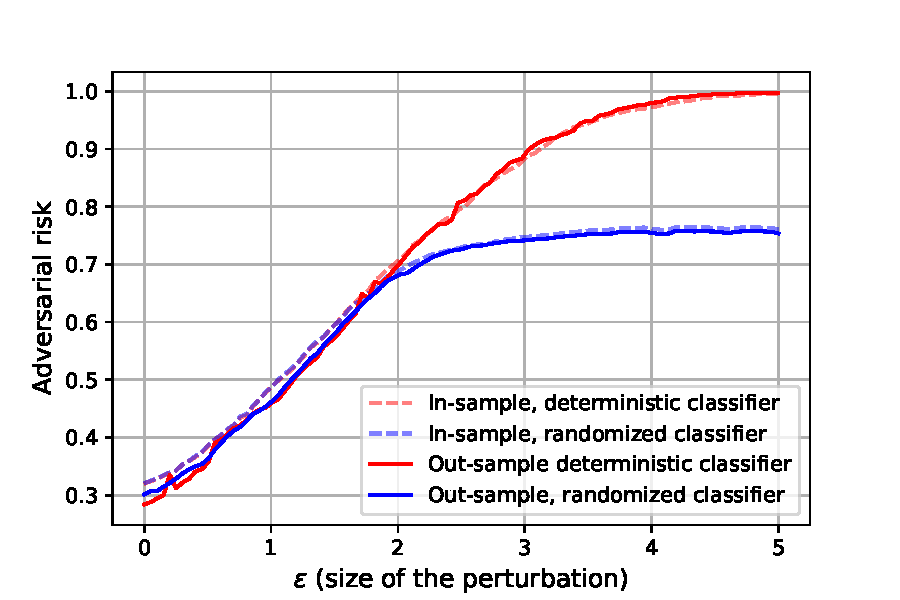
\includegraphics[width=0.32\textwidth]{Images/risk_toy.pdf}
    \caption{On left, $40$ data samples with their set of possible attacks represented in shadow and the optimal randomized classifier, with a color gradient representing the probability of the classifier. \textcolor{black}{In the middle}, convergence of the oracle ($\alpha=0$) and regularized algorithm for different values of regularization parameters. On right, in-sample and out-sample risk for randomized and deterministic minimum risk in function of the perturbation size $\varepsilon$. In the latter case, the randomized classifier is optimized with oracle Algorithm~\ref{algo:duchi}.}
    \label{fig:toy_example}
\end{figure*}


\textbf{An Entropic Relaxation.} Using the results from Section~\ref{sec:entropic-reg}, adding an entropic term to the objective allows to have a simple reformulation of the problem, as follows:
\begin{align*}
  \inf_{\bm{\lambda}\in \Delta_l}\sum_{i=1}^\numsamples  \frac{\varepsilon_i}{\numsamples}\log\left( \frac{1}{m_i}\sum_{j=1}^{m_i}\exp\left(\frac{\sum_{k=1}^l \lambda_k\loss(\theta_k,u_j^{(i)})}{\varepsilon_i}\right)\right)
\end{align*}
Note that in $\bm{\lambda}$, the objective is convex and smooth. One can  apply the accelerated PGD~\citep{beck2009fast,tseng2008accelerated} which enjoys an optimal convergence rate for first order methods of $\mathcal{O}(T^{-2})$ for $T$ iterations.

\textbf{A First Oracle Algorithm.} Indepedently from  the entropic regularization,we present an oracle-based algorithm inspired from~\citep{sinha2017certifying} and the convergence of projected sub-gradient methods~\citep{boyd2003subgradient}. The computation of the inner supremum problem is usually NP-hard. Let us justify it on a mixture of linear classifiers in binary classification: $f_{\theta_k,b_k}(x) = \langle \theta,x\rangle+b_k$ for $k\in [L]$ and $\bm{\lambda}=\mathbf{1}_L/L$. Let us consider the $\ell_2$ norm and $x=0$ and $y=1$. Then the problem of attacking $x$ is the following:
\begin{align*}
    \sup_{\tau,~\lVert \tau\rVert\leq\varepsilon} \frac{1}{L}\sum_{k=1}^L\mathbf{1}_{\langle \theta_k,x+\tau\rangle+b_k\leq0}
\end{align*}
This problem is equivalent to a linear binary classification problem on $\tau$, which is known to be NP-hard. Assuming the existence of a $\delta$-approximate oracle to this supremum, we algorithm is presented in Algorithm~\ref{algo:duchi}. We get the following guarantee for this algorithm. %See proof in Appendix~\ref{prv:algo-oracle}.
\begin{prop}
\label{prop:algo-oracle}
% Let $\PP\in\mathcal{M}^1_+(\mathcal{X}\times\mathcal{Y})$.
Let $\loss:\Theta\times(\mathcal{X}\times\mathcal{Y})\to [0,\infty)$ satisfying Assumption~\ref{ass:loss}. Then, Algorithm~\ref{algo:duchi} satisfies:  
\begin{align*}
    \min_{t\in[T]} \widehat{\mathcal{R}}_{adv}^{\varepsilon}(\bm{\lambda}_t)-\widehat{\mathcal{R}}_{adv}^{\varepsilon,*}\leq2\delta+\textcolor{black}{ \frac{2M\sqrt{l}}{\sqrt{T}}}
    % \delta\sqrt{K}+ \frac{M\sum_{t=1}^T \eta_t^2+\rVert\lambda_0-\lambda^*\lVert^2}{\sum_{t=1}^T\eta_t}
\end{align*}
% In particular for $\eta_t =\frac{\eta}{t^{1/2}}$, we get: $\min_{t\in[T]}\risk^\varepsilon(\lambda_t)-\risk^\varepsilon(\lambda^*)\in O\left(\delta+\frac{\log T}{\sqrt{T}}\right)$
\end{prop}

\begin{proof}
Thanks to Danskin theorem, if $\QQ^*$ is a best response to $\bm{\lambda}$, then $$\bm{g}^*:=\left(\mathbb{E}_{\QQ^*}\left[\loss(\theta_1,(x,y))\right],\dots,\mathbb{E}_{\QQ^*}\left[\loss(\theta_l,(x,y))\right]\right)^T$$ is a subgradient of $\bm{\lambda}\to \risk^\varepsilon(\bm{\lambda})$. Let $\eta\geq 0$ be the learning rate. Then we have for all $t\geq 1$:
\begin{align*}
\lVert \bm{\lambda}_t-\bm{\lambda}^*\rVert^2&\leq \lVert \bm{\lambda}_{t-1}-\eta \bm{g}_t-\bm{\lambda}^*\rVert^2\\
&=\lVert \bm{\lambda}_{t-1}-\bm{\lambda}^*\rVert^2-2\eta \langle\bm{g}_t, \bm{\lambda}_{t-1}-\bm{\lambda}^*\rangle+ \eta^2\lVert \bm{g}_t\rVert^2\\
&\leq \lVert \bm{\lambda}_{t-1}-\bm{\lambda}^*\rVert^2-2\eta \langle\bm{g}^*_t, \bm{\lambda}_{t-1}-\bm{\lambda}^*\rangle\\
&+2\eta\langle\bm{g}^*_t-\bm{g}_t, \bm{\lambda}_{t-1}-\bm{\lambda}^*\rangle+\eta^2 M^2 l\\
&\leq \lVert \bm{\lambda}_{t-1}-\bm{\lambda}^*\rVert^2-2\eta\left(\risk^\varepsilon(\bm{\lambda}_t)-\risk^\varepsilon(\bm{\lambda}^*)\right) +4\eta\delta+\eta^2  M^2 l%\lVert \bm{\lambda}_{t-1}-\bm{\lambda}^*\rVert_1
\end{align*}
We then deduce by summing:
\begin{align*}
   2\eta \sum_{t=1}^T \risk^\varepsilon(\bm{\lambda}_t)-\risk^\varepsilon(\bm{\lambda}^*) \leq 4\delta\eta T +\lVert \bm{\lambda}_{0}-\bm{\lambda}^*\rVert^2+\eta^2 M^2 lT
\end{align*}
Then we have:
\begin{align*}
    \min_{t\in[T]}\risk^\varepsilon(\bm{\lambda}_t)-\risk^\varepsilon(\bm{\lambda}^*)\leq 2\delta+\frac{4}{\eta T}+M^2l\eta
\end{align*}
The left-hand term is minimal for $\eta=\frac{2}{M\sqrt{lT}}$, and for this value:
\begin{align*}
    \min_{t\in[T]}\risk^\varepsilon(\bm{\lambda}_t)-\risk^\varepsilon(\bm{\lambda}^*)\leq 2\delta+\frac{2M\sqrt{l}}{\sqrt{T}}
\end{align*}
\end{proof}. 

The main drawback of the above algorithm is that one needs to have access to an oracle to guarantee the convergence of the proposed algorithm whereas its regularized version in order to approximate the solution and propose a simple algorithm to solve it.

 %In practice, we can change the distribution of sampling, to be more likely to find adversaries. 
% \begin{rmq}
% In general, one can use the exact same tools to obtain a proxy of the general DRO problem. Indeed thanks to~\citep{blanchet2019quantifying}, the dual can be approximated by adding an entropic term to the objective which leads to. We end-up with a minimization problem of a convex objective over the set of distribution. 
% \end{rmq}

\subsection{A General Heuristic Algorithm}

So far, our algorithms are not easily practicable in the case of deep learning. Adversarial examples are known to be easily transferrable from one model to another~\citep{tramer2017space,papernot2016transferability}. So we aim at learning diverse models. To this end, and support our theoretical claims, we propose an heuristic algorithm (see Algorithm~\ref{algo:heuristic}) to train a robust mixture of $l$ classifiers.   We alternatively train these classifiers with adversarial examples against the current mixture and update the probabilities of the mixture according to the algorithms we proposed in Section~\ref{sec:proposed-algo}. 


\begin{algorithm}[h!]
\SetAlgoLined
$l$: number of models, $T$: number of iterations,\\
$T_\theta$: number of updates for the models $\bm{\theta}$,\\
$T_\lambda$: number of updates for the mixture $\bm{\lambda}$,\\ $\bm{\lambda}_0=(\lambda_0^1,\dots\lambda_0^l),~\bm{\theta}_0=(\theta_0^1,\dots\theta_0^l)$\\
 \For{$t=1,\dots,T$}{
 Let $B_t$ be a batch of data.\\
\eIf{$t \mod (T_\theta l+1)\neq 0$}{
$k$ sampled uniformly in $\{1,\dots,l\}$\\
$\Tilde{B}_t\leftarrow$ Attack of images in $B_t$ for the  model $(\bm{\lambda}_t,\bm{\theta}_t)$\\
$\theta^t_k\leftarrow$ Update $\theta^{t-1}_k$ with $\Tilde{B}_t$ for fixed $\bm{\lambda}_t$ with a SGD step}{
$\bm{\lambda}_t\leftarrow$Update $\bm{\lambda}_{t-1}$ on $B_t$ for fixed $\bm{\theta}_t$
with oracle-based or regularized algorithm with $T_\lambda$ iterations.
}
  }
 \caption{Adversarial Training for Mixtures}
 
 \label{algo:heuristic}
\end{algorithm}
